 \documentclass[xcolor=x11names,compress]{beamer}

%% General document %%%%%%%%%%%%%%%%%%%%%%%%%%%%%%%%%%
\usepackage{graphicx}
\usepackage{tikz}
\usepackage{Tabbing}
\usetikzlibrary{decorations.fractals}
\usepackage{fancyvrb}
%%%%%%%%%%%%%%%%%%%%%%%%%%%%%%%%%%%%%%%%%%%%%%%%%%%%%%

%% Beamer Layout %%%%%%%%%%%%%%%%%%%%%%%%%%%%%%%%%%
\useoutertheme[subsection=false,shadow]{miniframes}
\useinnertheme{default}
\usefonttheme{serif}
\usepackage{palatino}
\usepackage{tabu}
% Links
\usepackage{hyperref}
\definecolor{links}{HTML}{003262}
\hypersetup{colorlinks,linkcolor=,urlcolor=links}

% addition of color
\usepackage{xcolor}
\definecolor{CoolBlack}{rgb}{0.0, 0.18, 0.39}
\definecolor{byellow}{rgb}{0.55037, 0.38821, 0.06142}
\definecolor{dgreen}{rgb}{0.,0.6,0.}
\definecolor{RawSienna}{cmyk}{0,0.72,1,0.45}
\definecolor{forestgreen(web)}{rgb}{0.13, 0.55, 0.13}
\definecolor{cardinal}{rgb}{0.77, 0.12, 0.23}

\setbeamerfont{title like}{shape=\scshape}
\setbeamerfont{frametitle}{shape=\scshape}

\setbeamercolor*{lower separation line head}{bg=CoolBlack}
\setbeamercolor*{normal text}{fg=black,bg=white}
\setbeamercolor*{alerted text}{fg=dgreen} % just testing; I think this looks better
\setbeamercolor*{example text}{fg=black}
\setbeamercolor*{structure}{fg=black}

\setbeamercolor*{palette tertiary}{fg=black,bg=black!10}
\setbeamercolor*{palette quaternary}{fg=black,bg=black!10}

% Margins
\usepackage{changepage}

\mode<presentation>
{
  \definecolor{berkeleyblue}{HTML}{003262}
  \definecolor{berkeleygold}{HTML}{FDB515}
  \usetheme{Boadilla}      % or try Darmstadt, Madrid, Warsaw, Boadilla...
  %\usecolortheme{dove} % or try albatross, beaver, crane, ...
  \setbeamercolor{structure}{fg=berkeleyblue,bg=berkeleygold}
  \setbeamercolor{palette primary}{bg=berkeleyblue,fg=white} % changed this
  \setbeamercolor{palette secondary}{fg=berkeleyblue,bg=berkeleygold} % changed this
  \setbeamercolor{palette tertiary}{bg=berkeleyblue,fg=white} % changed this
  \usefonttheme{structurebold}  % or try serif, structurebold, ...
  \useinnertheme{circles}
  \setbeamertemplate{navigation symbols}{}
  \setbeamertemplate{caption}[numbered]
  \usebackgroundtemplate{}
}

% Columns
\renewcommand{\(}{\begin{columns}}
\renewcommand{\)}{\end{columns}}
\newcommand{\<}[1]{\begin{column}{#1}}
\renewcommand{\>}{\end{column}}

\usepackage{cutwin}

% adding slide numbers
\addtobeamertemplate{navigation symbols}{}{%
    \usebeamerfont{footline}%
    \usebeamercolor[fg]{footline}%
    \hspace{1em}%
    \insertframenumber/\inserttotalframenumber
}

% equation stuff
\newcommand{\Macro}{\ensuremath{\Sigma}}
\newcommand{\Sn}{\ensuremath{S_N} }
\newcommand{\vOmega}{\ensuremath{\hat{\Omega}}}
\usepackage{mathrsfs}
\usepackage[mathcal]{euscript}
\usepackage{amssymb}
\usepackage{amsthm}
\usepackage{epsfig}
\usepackage{amsmath}
\newcommand{\ve}[1]{\ensuremath{\mathbf{#1}}}
\newcommand{\micro}{\ensuremath{\sigma}}
\newcommand{\detR}{\ensuremath{\Sigma}}

% title stuff for footer
\title{The PyNE Software Library}
\author{R.\ N.\ Slaybaugh}
\date{27 October 2014}

%%%%%%%%%%%%%%%%%%%%%%%%%%%%%%%%%%%%%%%%%%%%%%%%%%%%%%
\begin{document}



%%%%%%%%%%%%%%%%%%%%%%%%%%%%%%%%%%%%%%%%%%%%%%%%%%%%%%
%%%%%%%%%%%%%%%%%%%%%%%%%%%%%%%%%%%%%%%%%%%%%%%%%%%%%%
\begin{frame}
\title{The PyNE Software Library}
%\subtitle{}
\author{
        \includegraphics[height=2cm]{../bk-eps-converted-to}\\R.\ N.\ Slaybaugh \\ Univ.\ of Cal.\ Berkeley}

\date{Nuclear Data Week\\ 6 November 2014\\ Brookhaven National Laboratory}
\titlepage
\end{frame}

%------------------------------------------------------
%\begin{frame}{Outline}
%
%	\begin{columns}
%  	\begin{column}{0.5\textwidth}
%	    \begin{itemize}
%        \item PyNE \cite{pyne}: what is it?
%
%        (Python for Nuclear Engineering)
%        \item PyNE Demo
%        \item Current initiatives
%        \item PyNE as a research tool
%        \item Get involved!
%	    \end{itemize}
%  	\end{column}
% 	%
% 	\begin{column}{0.4\textwidth}
% 	   \begin{center}
% 	   \begin{figure}
%       
\includegraphics[height=4cm]{pyne-icon-big}
%	   \end{figure}
% 	   \end{center}
%  	\end{column}
%	\end{columns}
%
%\end{frame}

%%%%%%%%%%%%%%%%%%%%%%%%%%%%%%%%%%%%%%%%%%%%%%%%%%%%%%
%%%%%%%%%%%%%%%%%%%%%%%%%%%%%%%%%%%%%%%%%%%%%%%%%%%%%%
\section{PyNE \cite{pyne}: what is it?}
\begin{frame}{What is PyNE?}

    PyNE is \textcolor{dgreen}{the} open source nuclear engineering toolkit.
    \vspace*{1em}
    \begin{itemize}
    \item PyNE is a \textcolor{dgreen}{library of composable tools} used to build
    nuclear science and engineering applications
    \item It is \textcolor{dgreen}{permissively licensed} (2-clause BSD)
    \item It supports both a \textcolor{dgreen}{C++} and a \textcolor{dgreen}{Python} API
    \item The name `PyNE' is a bit of a misnomer since most of the code
    base is in C++ but most daily usage happens in Python
    \item \textcolor{dgreen}{v0.4} is the current, stable release
    \item As an organization, PyNE was born in April 2011
    (however, core parts of PyNE have existed since 2007)
    \end{itemize}

\end{frame}

%------------------------------------------------------
\begin{frame}{What are the Goals of PyNE?}

    \begin{columns}
    \begin{column}{0.45\textwidth}
        To help nuclear engineers:
        \begin{itemize}
        \item be more \alert{productive} (don't reinvent the wheel!)
        \item have the \alert{best solvers}
        \item have a \alert{clear and useful API}
        \item write really \alert{great code}
        \item \alert{teach} the next generation
        \end{itemize}
  	\end{column}
   	%
 	\begin{column}{0.45\textwidth}
 	   \begin{center}
 	   \begin{figure}
       
\includegraphics[height=2cm]{../figs/pyne-icon-big}
	   \end{figure}
 	   \end{center}
  	\end{column}
	\end{columns}

\end{frame}

%%%%%%%%%%%%%%%%%%%%%%%%%%%%%%%%%%%%%%%%%%%%%%%%%%%%%%
%%%%%%%%%%%%%%%%%%%%%%%%%%%%%%%%%%%%%%%%%%%%%%%%%%%%%%
\section{Demo}
\begin{frame}{What Can PyNE Do?}

    The idea is to be able to easily combine components and avoid redeveloping
    utilities someone else has developed.

    \begin{itemize}
    \item Nuclear data and cross-section reading/processing
    \item Material handling
    \item Canonical nuclide and reaction naming conventions
    \item Mesh operations
    \item MCNP and Serpent input/output parsing
    \item Fuel cycle functionality (transmutation, enrichment)
    \item There's more, and the list continues to grow
    \end{itemize}

\end{frame}

%%%%%%%%%%%%%%%%%%%%%%%%%%%%%%%%%%%%%%%%%%%%%%%%%%%%%%
%%%%%%%%%%%%%%%%%%%%%%%%%%%%%%%%%%%%%%%%%%%%%%%%%%%%%%
\section{Current initiatives}
\begin{frame}{What are we Working on Now?}

    The biggest push: \textcolor{dgreen}{V\&V} $\rightarrow$ methodically making PyNE compliant
    with the QA standards we've ratified, which are based on the ASME NQA-1 standards
    \cite{pyne_vnv}

    \vspace*{1 em}
    Many other items (large and small) in our ``ticket" list

    \begin{center}
 	\begin{figure}
 	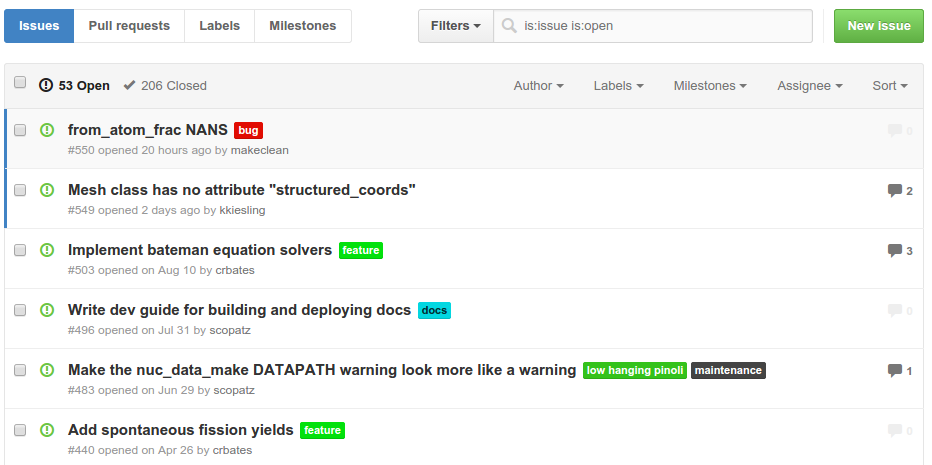
\includegraphics[height=1.75in,clip]{../figs/PyNE-tickets}
    \end{figure}
 	\end{center}

\end{frame}

%------------------------------------------------------
\begin{frame}{Verification and Validation}

    \textbf{Verification}: Have we built the software correctly?\\
    \textbf{Validation}: Have we built the correct software?

    \vspace*{1 em}
    Strategies employed by PyNE:

    \begin{itemize}
    \item Version control
    \item Formal review process
    \item Documentation: theory manual, user's guide, developer's guide, API,
    ticket system
    \item Test suite
    \item Continuous Integration
    \end{itemize}

\end{frame}
%%%%%%%%%%%%%%%%%%%%%%%%%%%%%%%%%%%%%%%%%%%%%%%%%%%%%%
%%%%%%%%%%%%%%%%%%%%%%%%%%%%%%%%%%%%%%%%%%%%%%%%%%%%%%
\begin{frame}{Nuclear Data in PyNE}
    \begin{itemize}
      \item ENSDF level and decay data
      \begin{itemize}
        \item parser
        \item conversion to hdf5
        \item access in c++ and Python
      \end{itemize}
      \item European Activation File cross sections
      \item Atomic mass data (KAERI)
      \item ENDF format cross section reader
      \item ACE format cross section reader
    \end{itemize}
\end{frame}


\begin{frame}{Nuclear Structure Data in PyNE}
    \begin{itemize}
      \item 177471 entries from IAEA ENSDF data
      \item spin, parity, energy level
      \item half-life, decay type, branching ratio
    \end{itemize}
\end{frame}

\begin{frame}{Nuclear Decay Data in PyNE}
    \begin{itemize}
      \item energy, intensity, initial and final levels for:
      \begin{itemize}
        \item 116598 gamma lines
        \item 13230 electron capture/beta +
        \item 11788 betas
        \item 2552 alphas
      \end{itemize}
      \item 3868 unique primary decays
    \end{itemize}
\end{frame}


%%%%%%%%%%%%%%%%%%%%%%%%%%%%%%%%%%%%%%%%%%%%%%%%%%%%%%
%%%%%%%%%%%%%%%%%%%%%%%%%%%%%%%%%%%%%%%%%%%%%%%%%%%%%%
\section{Get involved!}
\begin{frame}{Why Would I Get Involved?}

\begin{block}{As a \alert{user}:}
    \begin{itemize}
    \item You could do your work or research with PyNE
    \item Even if you have your own software that looks and behaves similarly to some aspects of PyNE, using PyNE will mean that you no longer have to develop AND maintain that functionality
    \end{itemize}
\end{block}

    \vspace*{1 em}
\begin{block}{As a \alert{developer}:}
    \begin{itemize}
    \item You should be selfish
    \item Contribute to PyNE in ways that support the work that you are doing
    \item If a feature you want is not in PyNE right now, chances are that other
    people want to see that feature too
    \item This will help your future self as much as future other people
    \end{itemize}
\end{block}

\end{frame}

%------------------------------------------------------
\begin{frame}{How Can I Get Involved?}

    \begin{block}{\alert{Contact PyNE}}
    \begin{itemize}
    \item Website: \href{http://pyne.io/}{\texttt{http://pyne.io/}}

    \item User's Mailing List: \href{pyne-users@googlegroups.com}
    {\texttt{pyne-users@googlegroups.com}}

    \item Developer's List: \href{pyne-dev@googlegroups.com}
    {\texttt{pyne-dev@googlegroups.com}}

    \item GitHub: \href{https://github.com/pyne/pyne}
    {\texttt{https://github.com/pyne/pyne}}

    \item Tutorial: \href{http://pyne.io/tutorial/index.html}
    {\texttt{http://pyne.io/tutorial/index.html}}

%    \begin{itemize}
%    \item Website: \url{http://pyne.io/}
%    \item User's Mailing List: \href{mailto:pyne-users@googlegroups.com}{\nolinkurl{pyne-users@googlegroups.com}}
%    \item Developer's List: \href{mailto:pyne-dev@googlegroups.com}{\nolinkurl{pyne-dev@googlegroups.com}}
%    \item GitHub: \url{https://github.com/pyne/pyne}
    \end{itemize}
    \end{block}

    \vspace*{2 em}
    \begin{block}{\alert{What goes into PyNE?}}
    Anything that is not export controllable, proprietary,
    or under HIPPA restrictions!  (If you have questions, \emph{ask})
    \end{block}

\end{frame}


%%%%%%%%%%%%%%%%%%%%%%%%%%%%%%%%%%%%%%%%%%%%%%%%%%%%%%
%%%%%%%%%%%%%%%%%%%%%%%%%%%%%%%%%%%%%%%%%%%%%%%%%%%%%%
\section*{}
\begin{frame}[fragile]{Questions?}

    \begin{center}
    \includegraphics[height=3in,clip]{../questions-comic}
    \end{center}

\end{frame}

% --------------------------------------------------------------
\begin{frame}[fragile]{PyNE In the Literature}

    \begin{itemize}
    \item Intro: ``PyNE: Python For Nuclear Engineering'' \cite{pyne_intro}
    \item Progress reports: \cite{scopatz_pyne}, \cite{pyne_progress}
    \item In research: \cite{Biondo2014}, \cite{MarquezDamian2014280}, \cite{Scopatz2013a}
    \item V\&V: ``Quality Assurance within the PyNE Open Source \\Toolkit'' \cite{pyne_vnv}
    \item Poster at SciPy: \cite{scipy}
    \end{itemize}

\end{frame}
% --------------------------------------------------------------
\begin{frame}[allowframebreaks]{References}
	\bibliographystyle{unsrt}
	\bibliography{2014-10-norcal-ans-pyne.bib}
\end{frame}

\end{document}
